\chapter{Web Server}

Analizzare le \textit{performance} di un \textit{web server}, effettuando le seguenti
attività:
\begin{itemize}
    \item \textbf{Capacity Test}: valutazione delle \textit{performance} del sistema al
    variare del carico di lavoro imposto;
    \item \textbf{Workload Characterization}: estrapolare un \textit{workload} sintetico
    a partire da un \textit{workload} reale e verificarne la significatività
    statistica dei rispettivi \textit{workload} di basso livello;
    \item \textbf{Design of Experiment}: verifica dell’influenza dei fattori sul
    \textit{response time} del sistema.
\end{itemize}

\section{Capacity Test}

Il web server è stato installato su una macchina virtuale \textit{VirtualBox} con le specifiche in \cref{tab:web_server_specs}. Le caratteristiche della macchina host sono mostrat in \cref{tab:host_specs}.

\begin{table}[H]
\centering
    \begin{tabular}{|c|p{0.3\linewidth}|}
    \hline
    \multicolumn{1}{|c|}{\textbf{Caratteristiche}} &
    \multicolumn{1}{c|}{\textbf{Server}}
    \tabularnewline \hline

CPU & 2 vCPU \tabularnewline \hline

RAM & 512 MB\tabularnewline \hline

OS & Alpine Linux 3.19, kernel 6.6.10-lts \tabularnewline \hline

Web server & Apache v2.4.58 \tabularnewline \hline
\end{tabular}
\caption{Tabella riassuntiva delle caratteristiche del Web Server}
\label{tab:web_server_specs}
\end{table}

\begin{table}[H]
\centering
    \begin{tabular}{|c|p{0.3\linewidth}|}
    \hline
    \multicolumn{1}{|c|}{\textbf{Caratteristiche}} &
    \multicolumn{1}{c|}{\textbf{Server}}
    \tabularnewline \hline

CPU & AMD Ryzen 5 2600, 6 core 12 threads \tabularnewline \hline

RAM & 16 GB, DDR4 3000 MHz\tabularnewline \hline

OS & Windows 10 \tabularnewline \hline
\end{tabular}
\caption{Tabella riassuntiva delle caratteristiche della macchina \textit{Host}}
\label{tab:host_specs}
\end{table}

Per il capacity test vengono prese in considerazione 2 metriche:
\begin{itemize}
    \item \textbf{Response Time}: intervallo di tempo che intercorre tra la richiesta
di una risorsa e la ricezione della risposta del sistema;
    \item \textbf{Throughput}: il numero di richieste per unità di tempo che
vengono servite dal server.
\end{itemize}

In particolare, sono state predisposte $10$ risorse di grandezza variabile da $64kB$ fino $1MB$.
Il capacity test ha come scopo quello di definire i punti di:
\begin{itemize}
    \item \textbf{Knee Capacity}: punto in cui la potenza (rapporto tra \textit{throughput}
    e \textit{response time}) è massima, dunque, rappresenta il miglior
    punto di funzionamento del sistema, poiché si ha il miglior tradeoff
    tra le due metriche adottate;
    \item \textbf{Usable Capacity}: punto in cui si ha il throughput massimo,
    senza superare i vincoli sul tempo di risposta. Dopo tale punto il
    throughput decresce al crescere del carico ed il tempo di risposta
    peggiora.
\end{itemize}
Attraverso uno script in \textit{Python} e il tool Jmeter, sono state raccolti campioni per livello di carico crescenti (regolando il valore \textit{Constant Throuhput Timer} (CTT)) effettuando 3 ripetezioni di ogni livello. 
Per assicurare l'indipendenza dei campioni è stato effettuato un riavvio del sistema tra una cattura e l'altra.
In particolare, è stata presa la media delle osservazioni come valore di riferimento per il campione ottenendo i dati in \cref{tab:capacity_results}. 
\begin{table}[H]

\centering
    \begin{tabular}{|c|c|c|}
    \hline
    \multicolumn{1}{|c|}{\textbf{CTT}} &
    \multicolumn{1}{|c|}{\textbf{Throughput (rps)}} &
    \multicolumn{1}{c|}{\textbf{Response time (millisecondi)}}  \tabularnewline \hline

200 & 3.56 & 72.96 \tabularnewline \hline
400 & 5.18 & 79.60 \tabularnewline \hline
600 & 4.93 & 113.71 \tabularnewline \hline
800 & 13.54 & 98.25 \tabularnewline \hline
1000 & 16.86 & 140.25 \tabularnewline \hline
1200 & 20.16 & 362.56 \tabularnewline \hline
1400 & 22.50 & 1901.10 \tabularnewline \hline
1600 & 18.35 & 3285.09 \tabularnewline \hline
\end{tabular}
\caption{Tabella riassuntiva delle caratteristiche dei due sistemi a cui è stato sottoposto il benchmark}
\label{tab:capacity_results}
\end{table}


\begin{figure}[H]
    \centering
    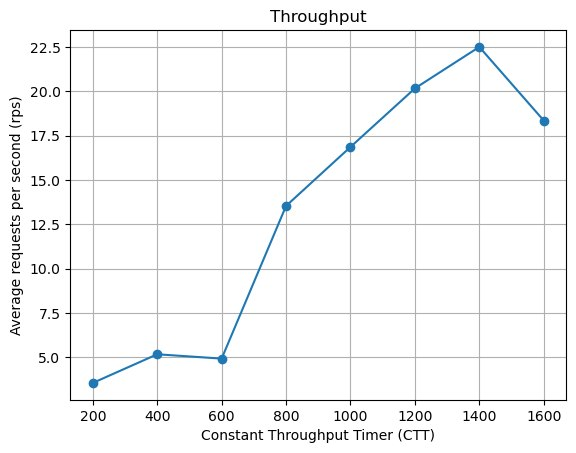
\includegraphics[width=0.8\textwidth]{img/ch3/throughput.jpeg}
    \caption{Throughput medio del web server al variare del carico}
    \label{fig:tput}
\end{figure}

\begin{figure}[H]
    \centering
    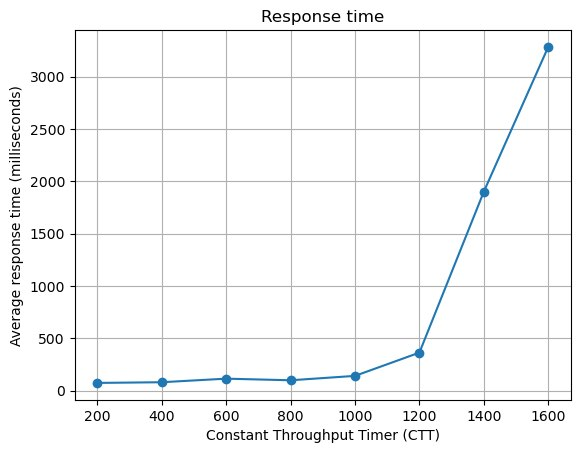
\includegraphics[width=0.8\textwidth]{img/ch3/responsetime.jpeg}
    \caption{Tempo di risposta medio del web server al variare del carico}
    \label{fig:responsetime}
\end{figure}

\begin{figure}[H]
    \centering
    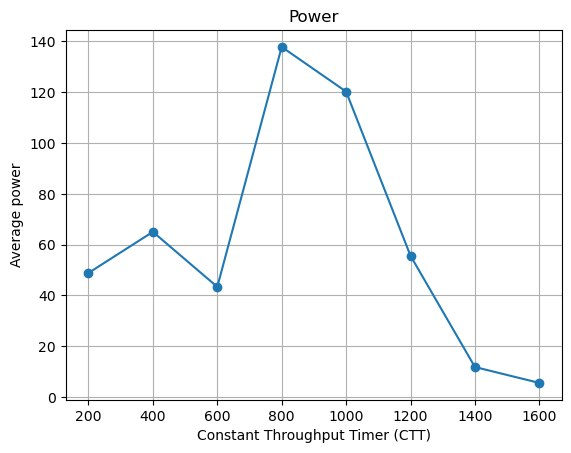
\includegraphics[width=0.8\textwidth]{img/ch3/power.jpeg}
    \caption{Andamento della potenza media del web server
    al variare del carico}
    \label{fig:power}
\end{figure}

A valle dei test svolti sono stati identificati i seguenti punti di interesse:
\begin{itemize}
    \item Knee Capacity: $800$ richieste al minuto;
    \item Usable capacity: $1400$ richieste al minuto;
\end{itemize}

\clearpage
\subsection{Bottleneck Performance}

Ai fini di identificare le risorse del sistema sottoposte a \textit{stress} maggiore sono state monitorate le risorse sul server con l'utility \textit{vmstat}. Analogamente ai parametri di alto livello, anche i parametri di sistema sono stati catturati effettuando $3$ osservazioni prendendo la media per ciascun punto. Tra le risorse monitorate sono presenti:
\begin{itemize}
    \item Utilizzo CPU;
    \item Numero di \textit{context switch};
    \item Consumo di memoria;
    \item Numero di interruzioni al secondo;
    \item \textit{Byte} inviati al secondo (kb/s);
\end{itemize}


In \cref{fig:low_level_parameters_cpu}, \cref{fig:low_level_parameters_mem}  e \cref{fig:low_level_io}, sono mostrati i grafici relativi agli andamenti medi dell'utilizzo del processore e della memoria e i parametri relativi alle prestazioni di I/O. 

\begin{figure}[H]
    \centering
    \begin{subfigure}{0.5\textwidth}
        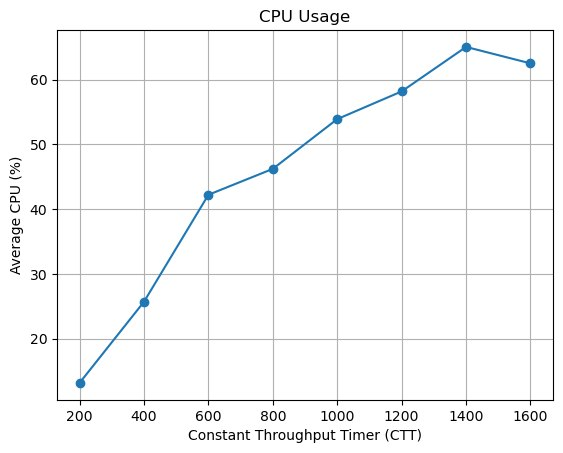
\includegraphics[width=0.95\linewidth]{img/ch3/cpu.jpeg}
        \caption{Andamento utilizzo medio CPU}
    \end{subfigure}\hfil
    \begin{subfigure}{0.5\textwidth}
        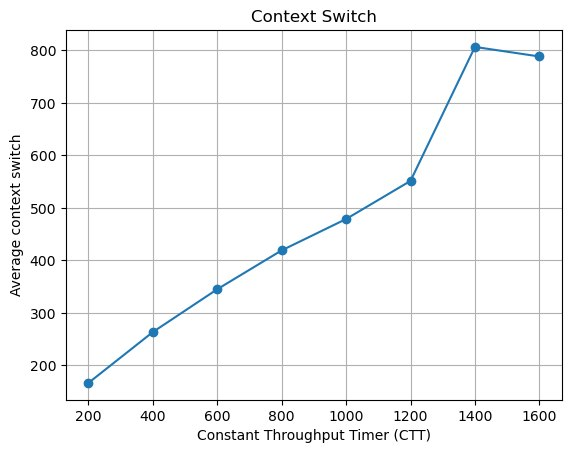
\includegraphics[width=0.95\linewidth]{img/ch3/contextswitch.jpeg}
        \caption{Numero medio di context switch}
    \end{subfigure}
    \caption{Andamento utilizzazione del processore e cambi di contesto}
    \label{fig:low_level_parameters_cpu}
\end{figure}

\begin{figure}[H]
    \centering
    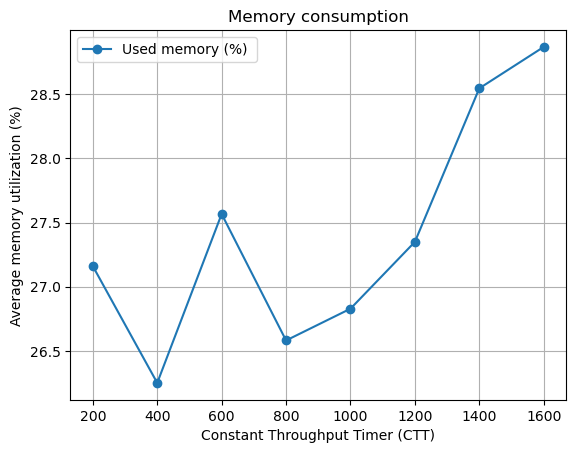
\includegraphics[width=0.6\linewidth]{img/ch3/mem.png}
    \caption{Andamento memoria utilizzata}
    \label{fig:low_level_parameters_mem}
\end{figure}

\begin{figure}[H]
    \centering
    \begin{subfigure}{0.5\textwidth}
        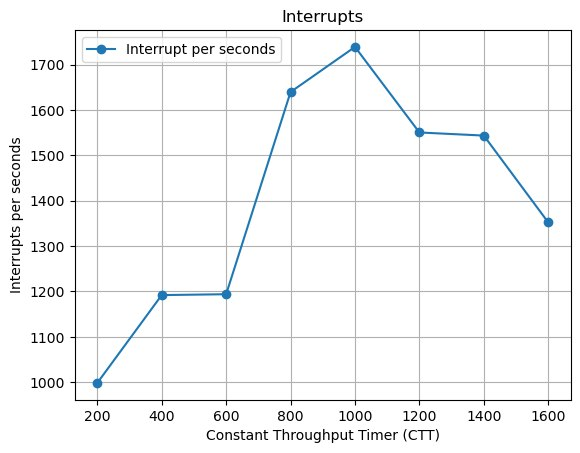
\includegraphics[width=0.95\linewidth]{img/ch3/interrupts.jpeg}
        \caption{Numero medio di interruzioni al secondo}
    \end{subfigure}\hfil
    \begin{subfigure}{0.5\textwidth}
        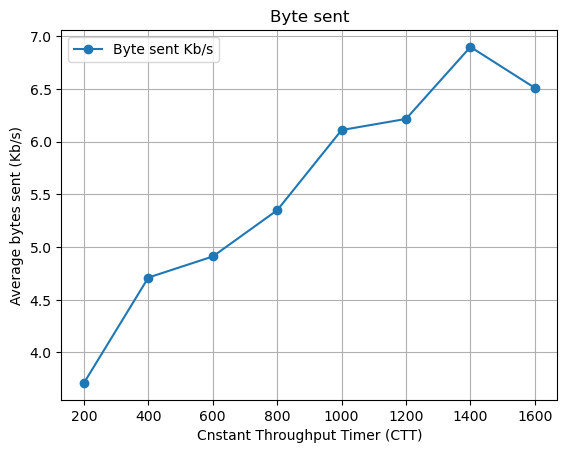
\includegraphics[width=0.95\linewidth]{img/ch3/byte_sent.png}
        \caption{Byte inviati al secondo (kb/s)}
    \end{subfigure}
    \caption{Andamento parametri riguardanti l'I/O}
    \label{fig:low_level_io}
\end{figure}


In particolare, si osserva che la saturazione del sistema che avviene dal  $CTT = 1400$, corrispondente al punto di \textit{usable capacity}, sembra essere causata dall'alto utilizzo della CPU. In figura \cref{fig:cpuvsmem} sono mostrate le percentuali di utilizzo di memoria e CPU messe a confronto, dove risulta chiaro che quest'ultima è il bottleneck.

\begin{figure}[H]
    \centering
    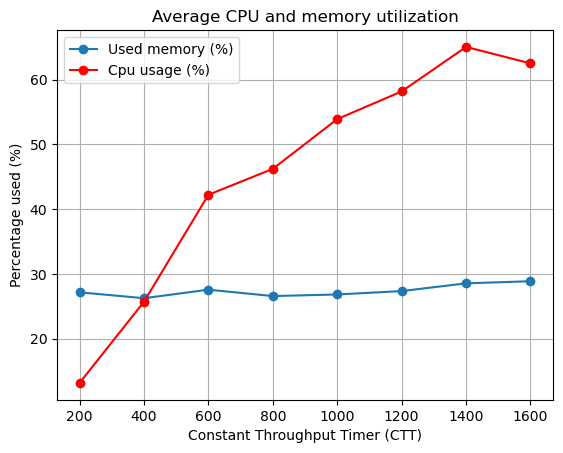
\includegraphics[width=0.8\linewidth]{img/ch3/cpu_vs_mem.png}
    \caption{Confronto percentuali di utilizzo di CPU e Memoria}
    \label{fig:cpuvsmem}
\end{figure}


\clearpage
\subsection{Fairness Index}

Si vuole valutare quanto il sistema sia equo nell'assegnazione delle risorse a più gruppi di utenti concorrenti. 
Per farlo, si calcola il \textit{Fairness Index} definito nella \cref{eq:fairness_index}.

\begin{equation}
    f = \frac{\left(\sum \limits _{i=1}^n x_i\right)^2}{n \cdot \sum \limits _{i=1}^n x_i^2}
    \label{eq:fairness_index}
\end{equation}

Sono stati creati i seguenti thread group su \textit{jmeter} per simulare l'attività degli utenti:

\begin{itemize}
    \item TG1: composto da $20$ utenti che fanno richieste leggere;
    \item TG2: composto da $15$ utenti che fanno richieste medie;
    \item TG3: composto da $5$ utenti che fanno richieste pesanti;  
\end{itemize}

Dopo aver somministrato il test al \textit{server}, è stata effettuata la misura del \textit{throughput} reale in base a ciascun \textit{thread group}. In particolare sono stati ottenuti i risultati in \cref{tab:fairness_results}.

\begin{table}[H]
\centering
    \begin{tabular}{|c|r|r|r|}
    \hline
    \multicolumn{1}{|c|}{\textbf{Thread group ID}} &
    \multicolumn{1}{|c|}{\textbf{TTP Ideale}} &
    \multicolumn{1}{|c|}{\textbf{TTP Misurato}}  &
    \multicolumn{1}{|c|}{\textbf{TTP Normalizzato}}
    \tabularnewline \hline

TG1 & $3.33$ & $3.38$ & $1.016$ \tabularnewline \hline
TG2 & $3.33$ & $3.38$ & $1.013$ \tabularnewline \hline
TG3 & $6.67$ & $6.54$ & $0.980$ \tabularnewline \hline

\end{tabular}
\caption{Tabella riassuntiva per il calcolo del \textit{fairness index} (con \textit{TTP} si è indicato il \textit{througphut}, espresso in richieste al secondo)}

\label{tab:fairness_results}
\end{table}

Il throughput normalizzato si calcola con la seguente formula:
\begin{equation*}
 T_{norm} = \frac{T_{misurato}}{T_{ideale}}
\end{equation*}

Applicando la \cref{eq:fairness_index}, è stato calcolato il \textit{fairness index} con un valore pari a $0.9997$.

\clearpage
\section{Workload characterization}

La \textit{Workload Characterization} ha lo scopo di generare un \textit{workload} sintetico partendo da uno reale. Sono state svolte le seguenti fasi, illustrate in \cref{fig:charcterization_flow}:
\begin{itemize}
    \item Creazione del \textit{workload} reale di di alto livello ($HL$ \textit{High Level}) e di basso livello ($LL$ \textit{Low Level});
    \item Creazione del \textit{workload} sintetico tramite la caratterizzazione di HL ($HL_c$) e di LL ($LL_c$);
    \item Applicazione del \textit{workload} $HL_c$ per raccogliere i parametri di basso livello $LL'$;
    \item caratterizzazione del \textit{workload} $LL \rightarrow LL_c$;
    \item Verifica della bontà della caratterizzazione del \textit{workload} di alto livello tramite test di ipotesi dei parametri di basso livello caratterizzati $LL'_c \rightarrow LL'_c$;
\end{itemize}

\begin{figure}[H]
    \centering
    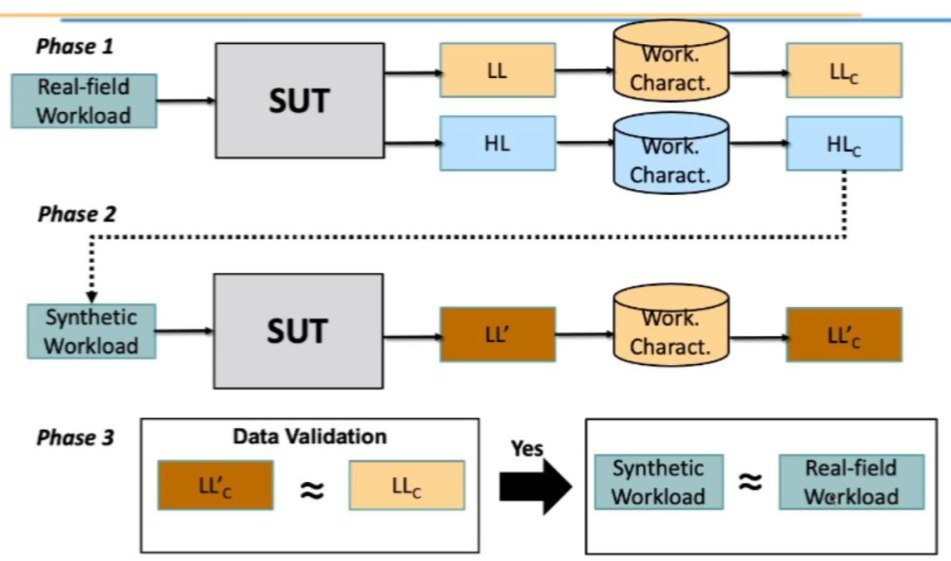
\includegraphics[width=0.8\textwidth]{img/ch3/characterization.jpg}
    \caption{Workload Characterization}
    \label{fig:charcterization_flow}
\end{figure}

\subsection{Workload reale}
Attraverso \textit{Jmeter} è stata generata una traccia di traffico reale con il \textit{web server} configurato per avere $20$ risorse di dimensione variabile da $64 kB$ a $3 MB$. Inoltre, è stata ipotizzata la presenza di $5$ gruppi di utenti distinti aventi accesso solo a $10$ risorse. I gruppi sono stati configurati secondo la \cref{tab:wc_real}. Ciascun gruppo di utenti effettua richieste per $5$ minuti.


\begin{table}[H]
\centering
    \begin{tabular}{|c|c|c|}
    \hline
    \multicolumn{1}{|c|}{\textbf{Thread group ID}} &
    \multicolumn{1}{|c|}{\textbf{Numero utenti}} &
    \multicolumn{1}{|c|}{\textbf{Richieste al minuto (CTT)}}
    \tabularnewline \hline

TG1 & $20$ & $400$ \tabularnewline \hline
TG2 & $15$ & $500$ \tabularnewline \hline
TG3 & $10$ & $600$ \tabularnewline \hline
TG4 & $25$ & $200$ \tabularnewline \hline
TG5 & $40$ & $150$ \tabularnewline \hline
\end{tabular}
\caption{Tabella riassuntiva per la generazione della traccia di traffico reale}

\label{tab:wc_real}
\end{table}

Inoltre, durante la generazione della traccia di traffico reale sono stati collezionati parametri di basso livello sul server attraverso l'\textit{utility} \textit{vmstat}.

In \cref{tab:tg1_real}, sono riportate le richieste effettuate dal \textit{TG1}.

\begin{table}[H]
\centering
    \begin{tabular}{|c|c|c|}
    \hline
    \multicolumn{1}{|c|}{\textbf{Risorsa}} &
    \multicolumn{1}{|c|}{\textbf{Nome}} &
    \multicolumn{1}{|c|}{\textbf{Dimensione}}
    \tabularnewline \hline

1 & 1.png & 64 KB \tabularnewline \hline
2 & 5.pdf & 452 KB \tabularnewline \hline
3 & 10.pdf & 771 KB \tabularnewline \hline
4 & 15.pdf & 1.3 MB \tabularnewline \hline
5 & 17.pdf & 1.7 MB \tabularnewline \hline
6 & 2.html & 127 KB \tabularnewline \hline
7 & 11.pdf & 857 KB \tabularnewline \hline
8 & 19.pdf & 2.6 MB \tabularnewline \hline
9 & 4.png & 374 KB \tabularnewline \hline
10 & 8.pdf & 588 KB \tabularnewline \hline
\end{tabular}
\caption{Richieste effettuate da TG1}
\label{tab:tg1_real}
\end{table}

In \cref{tab:tg2_real}, sono riportate le richieste effettuate dal \textit{TG2}.

\begin{table}[H]
\centering
    \begin{tabular}{|c|c|c|}
    \hline
    \multicolumn{1}{|c|}{\textbf{Risorsa}} &
    \multicolumn{1}{|c|}{\textbf{Nome}} &
    \multicolumn{1}{|c|}{\textbf{Dimensione}}
    \tabularnewline \hline

1 & 3.docx & 230 KB   \tabularnewline \hline
2 & 7.pdf & 581 KB  \tabularnewline \hline
3 & 10.pdf & 771 KB \tabularnewline \hline
4 & 14.pdf & 1.2 MB \tabularnewline \hline
5 & 18.pdf & 2.1 MB \tabularnewline \hline
6 & 20.pdf & 2.9 MB \tabularnewline \hline
7 & 6.pdf & 528 KB  \tabularnewline \hline
8 & 11.pdf & 857 KB \tabularnewline \hline
9 & 16.pdf & 1.7 MB \tabularnewline \hline
10 & 2.html & 127 KB \tabularnewline \hline
\end{tabular}
\caption{Richieste effettuate da TG2}
\label{tab:tg2_real}
\end{table}

In \cref{tab:tg3_real}, sono riportate le richieste effettuate dal \textit{TG3}.

\begin{table}[H]
\centering
    \begin{tabular}{|c|c|c|}
    \hline
    \multicolumn{1}{|c|}{\textbf{Risorsa}} &
    \multicolumn{1}{|c|}{\textbf{Nome}} &
    \multicolumn{1}{|c|}{\textbf{Dimensione}}
    \tabularnewline \hline

1 & 7.pdf & 64 KB \tabularnewline \hline
2 & 17.pdf & 1.7 MB \tabularnewline \hline
3 & 13.pdf & 995 KB \tabularnewline \hline
4 & 9.pdf & 659 KB \tabularnewline \hline
5 & 4.png & 374 KB \tabularnewline \hline
6 & 18.pdf & 2.1 MB \tabularnewline \hline
7 & 12.pdf & 881 KB \tabularnewline \hline
8 & 6.pdf & 528 KB \tabularnewline \hline
9 & 14.pdf & 1.2 MB \tabularnewline \hline
10 & 19.pdf & 771 KB \tabularnewline \hline
\end{tabular}
\caption{Richieste effettuate da TG3}
\label{tab:tg3_real}
\end{table}

In \cref{tab:tg4_real}, sono riportate le richieste effettuate dal \textit{TG4}.
\begin{table}[H]
\centering
    \begin{tabular}{|c|c|c|}
    \hline
    \multicolumn{1}{|c|}{\textbf{Risorsa}} &
    \multicolumn{1}{|c|}{\textbf{Nome}} &
    \multicolumn{1}{|c|}{\textbf{Dimensione}}
    \tabularnewline \hline

1 & 4.png & 374 KB  \tabularnewline \hline
2 & 14.pdf & 1.2 MB \tabularnewline \hline
3 & 2.html & 127 KB  \tabularnewline \hline
4 & 12.pdf & 881 KB \tabularnewline \hline
5 & 9.pdf & 659 KB  \tabularnewline \hline
6 & 6.pdf & 528 KB  \tabularnewline \hline
7 & 2.html & 127 KB  \tabularnewline \hline
8 & 15.pdf & 1.3 MB \tabularnewline \hline
9 & 18.pdf & 2.1 MB \tabularnewline \hline
10 & 7.pdf & 581 KB \tabularnewline \hline
\end{tabular}
\caption{Richieste effettuate da TG4}
\label{tab:tg4_real}
\end{table}

In \cref{tab:tg5_real}, sono riportate le richieste effettuate dal \textit{TG5}.
\begin{table}[H]
\centering
    \begin{tabular}{|c|c|c|}
    \hline
    \multicolumn{1}{|c|}{\textbf{Risorsa}} &
    \multicolumn{1}{|c|}{\textbf{Nome}} &
    \multicolumn{1}{|c|}{\textbf{Dimensione}}
    \tabularnewline \hline

1 & 3.docx & 230 KB \tabularnewline \hline
2 & 7.pdf & 581 KB \tabularnewline \hline
3 & 9.pdf & 659 KB \tabularnewline \hline
4 & 4.png & 374 KB \tabularnewline \hline
5 & 15.pdf & 1.3 MB \tabularnewline \hline
6 & 11.pdf & 857 KB \tabularnewline \hline
7 & 4.png & 374 KB \tabularnewline \hline
8 & 12.pdf & 588 KB \tabularnewline \hline
9 & 4.png & 374 KB \tabularnewline \hline
10 & 19.pdf & 771 KB \tabularnewline \hline

\end{tabular}
\caption{Richieste effettuate da TG5}
\label{tab:tg5_real}
\end{table}

\subsection{Caratterizzazione del \textit{workload} reale}

\paragraph{Parametri di alto livello ($HL \rightarrow HL_c$)}
Terminata la fase di cattura, è stato caratterizzato il \textit{file csv} prodotto da \textit{jmeter} attraverso le operazioni di \textit{PCA} e \textit{Clustering}. In particolare, escluse le colonne non numeriche, sono state scelte $4$ componenti principali mantenendo circa il $95\%$ di devianza del \textit{dataset} iniziale. Successivamente, sono stati scelti $30$ cluster per raggruppare le richieste del \textit{workload} reale. In particolare, per ogni cluster è stata scelta la richiesta più rappresentativa (quella che compare un numero maggiore di volte) e in caso di sovrapposizione si è proceduto a scegliere le successive. In questo modo, mantenendo l'$89\%$ della devianza iniziale, si è passati da $50$ tipi di richieste a $30$ semplificando il \textit{workload iniziale} del $40\%$.


In \cref{tab:tg1_synthetic}, sono riportate le richieste effettuate dal \textit{TG1}.

\begin{table}[H]
\centering
    \begin{tabular}{|c|c|c|}
    \hline
    \multicolumn{1}{|c|}{\textbf{Risorsa}} &
    \multicolumn{1}{|c|}{\textbf{Nome}} &
    \multicolumn{1}{|c|}{\textbf{Dimensione}}
    \tabularnewline \hline

2 & 5.pdf & 452 KB \tabularnewline \hline
3 & 10.pdf & 771 KB \tabularnewline \hline
4 & 15.pdf & 1.3 MB \tabularnewline \hline
5 & 17.pdf & 1.7 MB \tabularnewline \hline
7 & 11.pdf & 857 KB \tabularnewline \hline
8 & 19.pdf & 2.6 MB \tabularnewline \hline
9 & 4.png & 374 KB \tabularnewline \hline
\end{tabular}
\caption{Richieste effettuate da TG1 per il workload sintetico}
\label{tab:tg1_synthetic}
\end{table}

In \cref{tab:tg2_synthetic}, sono riportate le richieste effettuate dal \textit{TG2}.

\begin{table}[H]
\centering
    \begin{tabular}{|c|c|c|}
    \hline
    \multicolumn{1}{|c|}{\textbf{Risorsa}} &
    \multicolumn{1}{|c|}{\textbf{Nome}} &
    \multicolumn{1}{|c|}{\textbf{Dimensione}}
    \tabularnewline \hline

1 & 3.docx & 230 KB   \tabularnewline \hline
2 & 7.pdf & 581 KB  \tabularnewline \hline
3 & 10.pdf & 771 KB \tabularnewline \hline
4 & 14.pdf & 1.2 MB \tabularnewline \hline
5 & 18.pdf & 2.1 MB \tabularnewline \hline
6 & 20.pdf & 2.9 MB \tabularnewline \hline
7 & 6.pdf & 528 KB  \tabularnewline \hline
8 & 11.pdf & 857 KB \tabularnewline \hline
9 & 16.pdf & 1.7 MB \tabularnewline \hline
10 & 2.html & 127 KB \tabularnewline \hline
\end{tabular}
\caption{Richieste effettuate da TG2 per il workload sintetico}
\label{tab:tg2_synthetic}
\end{table}

In \cref{tab:tg3_synthetic}, sono riportate le richieste effettuate dal \textit{TG3}.

\begin{table}[H]
\centering
    \begin{tabular}{|c|c|c|}
    \hline
    \multicolumn{1}{|c|}{\textbf{Risorsa}} &
    \multicolumn{1}{|c|}{\textbf{Nome}} &
    \multicolumn{1}{|c|}{\textbf{Dimensione}}
    \tabularnewline \hline

1 & 7.pdf & 64 KB \tabularnewline \hline
2 & 17.pdf & 1.7 MB \tabularnewline \hline
3 & 13.pdf & 995 KB \tabularnewline \hline
4 & 9.pdf & 659 KB \tabularnewline \hline
6 & 18.pdf & 2.1 MB \tabularnewline \hline
7 & 12.pdf & 881 KB \tabularnewline \hline
8 & 6.pdf & 528 KB \tabularnewline \hline
9 & 14.pdf & 1.2 MB \tabularnewline \hline
10 & 19.pdf & 771 KB \tabularnewline \hline
\end{tabular}
\caption{Richieste effettuate da TG3 per il workload sintetico}
\label{tab:tg3_synthetic}
\end{table}

In \cref{tab:tg4_synthetic}, sono riportate le richieste effettuate dal \textit{TG4}.
\begin{table}[H]
\centering
    \begin{tabular}{|c|c|c|}
    \hline
    \multicolumn{1}{|c|}{\textbf{Risorsa}} &
    \multicolumn{1}{|c|}{\textbf{Nome}} &
    \multicolumn{1}{|c|}{\textbf{Dimensione}}
    \tabularnewline \hline

3 & 2.html & 127 KB  \tabularnewline \hline
\end{tabular}
\caption{Richieste effettuate da TG4 per il workload sintetico}
\label{tab:tg4_synthetic}
\end{table}

In \cref{tab:tg5_synthetic}, sono riportate le richieste effettuate dal \textit{TG5}.
\begin{table}[H]
\centering
    \begin{tabular}{|c|c|c|}
    \hline
    \multicolumn{1}{|c|}{\textbf{Risorsa}} &
    \multicolumn{1}{|c|}{\textbf{Nome}} &
    \multicolumn{1}{|c|}{\textbf{Dimensione}}
    \tabularnewline \hline

1 & 3.docx & 230 KB \tabularnewline \hline
5 & 15.pdf & 1.3 MB \tabularnewline \hline
10 & 19.pdf & 771 KB \tabularnewline \hline

\end{tabular}
\caption{Richieste effettuate da TG5 per il workload sintetico}
\label{tab:tg5_synthetic}
\end{table}

\paragraph{Parametri di basso livello ($LL \rightarrow LL_c$)}
Similmente a quanto fatto per i parametri di alto livello, sono stati effettuati $PCA$ e $Clustering$ per i dati raccolti con \textit{vmstat}. In particolare, sono state scelte $6$ componenti principali e $20$ cluster perdendo circa il $13\%$ di devianza totale. Inoltre, in preparazione al test di ipotesi sono state verificate la normalità e l'omoschedasticità per le componenti principali calcolate.

\begin{figure}[H]
    \centering
    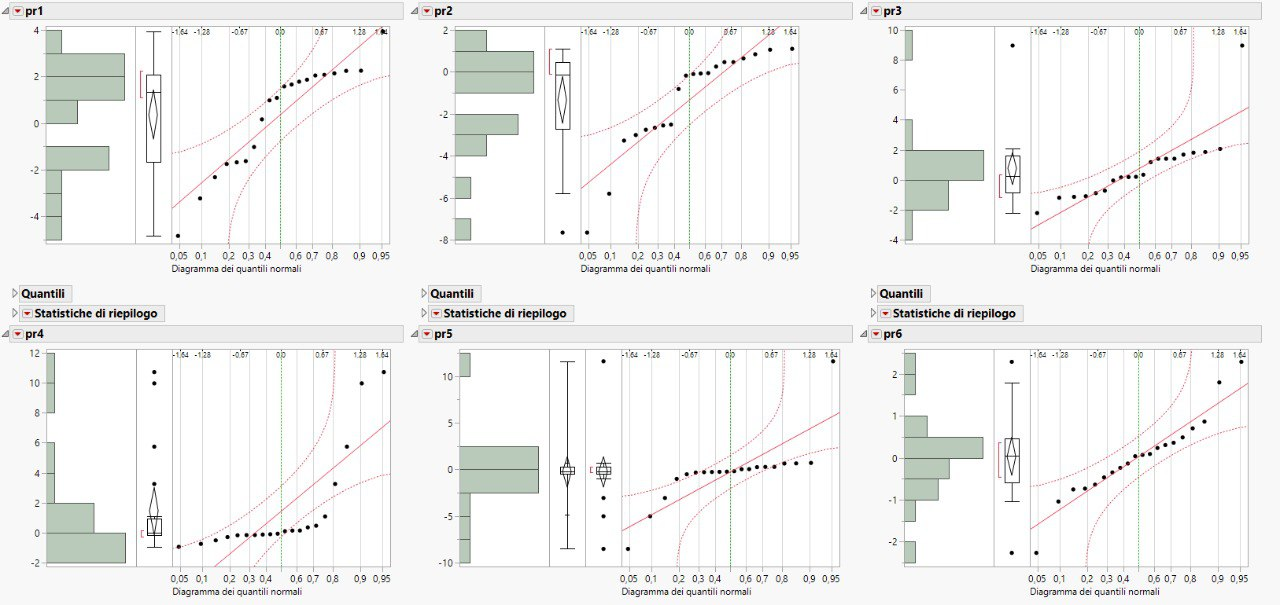
\includegraphics[width=\textwidth]{img/ch3/real.jpg}
    \caption{Test di normalità visivo delle componenti principali. Le componenti $1,2,3,6$ risultano normali.}
    \label{fig:real_qqplot}
\end{figure}

In \cref{fig:real_qqplot}, si osserva come le componente principali $1,2,3,6$ sembrano seguire la distribuzione normale, dato che i quantili sono all'interno delle bande. Tuttavia, data la presenza di alcuni punti in prossimità delle bande, si è scelto di procedere con il test di Shapiro-Wilk i cui risultati sono riportati in
\cref{tab:ll_norm}.

\begin{table}[H]
\centering
    \begin{tabular}{|c|c|r|}
    \hline
    \multicolumn{1}{|c|}{\textbf{Componente principale}} &
    \multicolumn{1}{|c|}{\textbf{Esito Shapiro-Wilk}} &
    \multicolumn{1}{|c|}{\textbf{P-value}}
    \tabularnewline \hline

1 & 0 & 0.053 \tabularnewline \hline
2 & 1 & 0.005 \tabularnewline \hline
3 & 1 & 0.0002 \tabularnewline \hline
6 & 0 & 0.485 \tabularnewline \hline
\end{tabular}
\caption{Risultati test normalità per le componenti $1,2,3,6$}
\label{tab:ll_norm}
\end{table}

È stata dimostrata l'omoschedasticità mediante il \textit{Two-sample F-test} in \cref{tab:ll_omoschedasticit} per le componenti $1,6$ risultate normali dal test precedente.

\begin{table}[H]
\centering
    \begin{tabular}{|c|c|r|}
    \hline
    \multicolumn{1}{|c|}{\textbf{Componente principale}} &
    \multicolumn{1}{|c|}{\textbf{Esito (H)}} &
    \multicolumn{1}{|c|}{\textbf{P-value}}
    \tabularnewline \hline

1 & 0 & 0.7227 \tabularnewline \hline
6 & 0 & 0.5020 \tabularnewline \hline
\end{tabular}
\caption{Risultati omoschedasticità componenti $1,6$}
\label{tab:ll_omoschedasticit}
\end{table}

\subsection{Validazione del workload sintetico ($LL' \rightarrow LL'_c$)}
Generato il \textit{workload} sintetico, questo è stato applicato al server collezionando nuovamente i parametri di basso livello ($LL'$) con \textit{vmstat}. Quindi si sono calcolate le $6$ componenti principali e si è effettuato il raggruppamento delle richieste in $20$ cluster, in maniera analoga a $LL_c$, ottenendo $LL'_c$.

\begin{figure}[H]
    \centering
    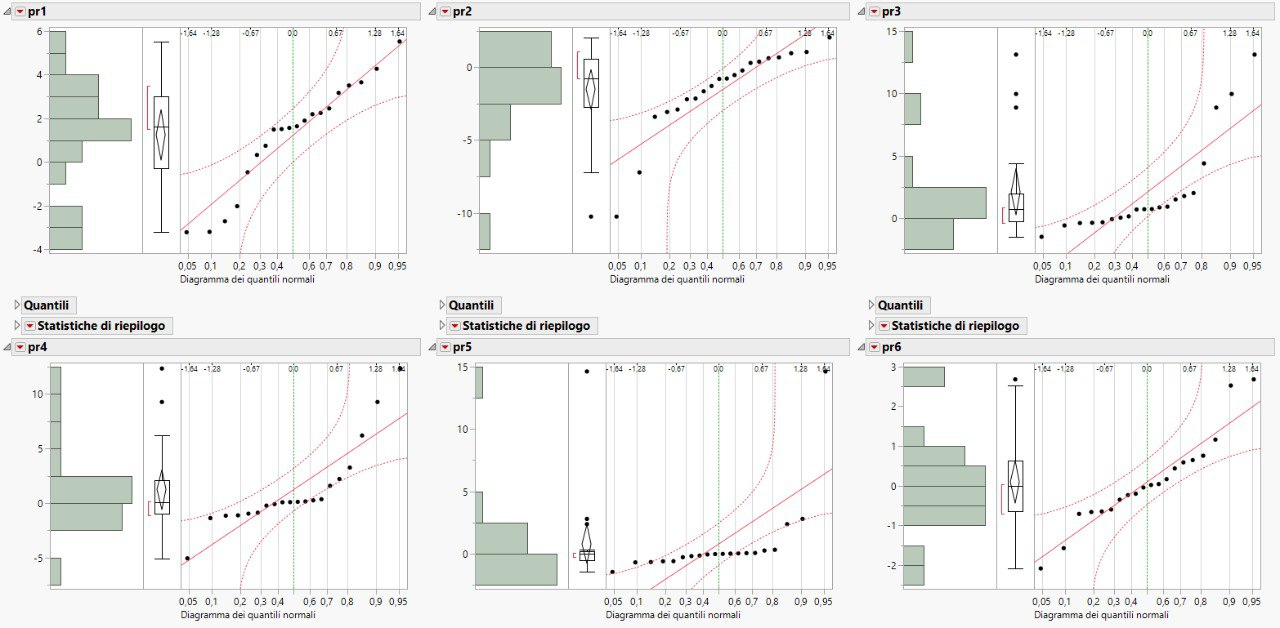
\includegraphics[width=\textwidth]{img/ch3/synth.jpg}
    \caption{Test di normalità visivo delle componenti principali.}
    \label{fig:synt_qqplot}
\end{figure}

Per le componenti $1,6$ è stata verificata la normalità sia visivamente che con il test di Shapiro-Wilk i cui
risultati sono messi in \cref{tab:ll1_norm}.
\begin{table}[H]
\centering
    \begin{tabular}{|c|c|r|}
    \hline
    \multicolumn{1}{|c|}{\textbf{Componente principale}} &
    \multicolumn{1}{|c|}{\textbf{Esito Shapiro-Wilk}} &
    \multicolumn{1}{|c|}{\textbf{P-value}}
    \tabularnewline \hline

1 & 0 & 0.218 \tabularnewline \hline
6 & 0 & 0.212 \tabularnewline \hline
\end{tabular}
\caption{Risultati test normalità per le componenti $1,6$}
\label{tab:ll1_norm}
\end{table}

È stata poi verificata l'omoschedasticità attraverso il \textit{Two-sample F-test} (\cref{tab:ll1_omoschedasticit}).

\begin{table}[H]
\centering
    \begin{tabular}{|c|c|r|}
    \hline
    \multicolumn{1}{|c|}{\textbf{Componente principale}} &
    \multicolumn{1}{|c|}{\textbf{Esito (H)}} &
    \multicolumn{1}{|c|}{\textbf{P-value}}
    \tabularnewline \hline

1 & 0 & 0.6487 \tabularnewline \hline
6 & 0 & 0.7826 \tabularnewline \hline
\end{tabular}
\caption{Risultati omoschedasticità componenti $1,6$}
\label{tab:ll1_omoschedasticit}
\end{table}


\paragraph{Test di ipotesi} Infine, si è proceduto nell'applicazione del test di ipotesi per ciascuna componente principale. Visti i risultati in \cref{tab:validation_test}, è possibile quindi concludere che non ci sono differenze statistiche tra il \textit{workload} sintetico e quello reale da cui si è partiti.

\begin{table}[H]
\centering
    \begin{tabular}{|c|c|c|r|}
    \hline
    \multicolumn{1}{|c|}{\textbf{Componenti principali}} &
    \multicolumn{1}{|c|}{\textbf{Tipologia di test}} &
    \multicolumn{1}{|c|}{\textbf{Esito(H)}} &
    \multicolumn{1}{|c|}{\textbf{P-value}}
    \tabularnewline \hline

PR1 & T-Test Equal Variance  & 0 & 0.0595 \tabularnewline \hline
PR2 & Wilcoxon rank sum  & 0 & 0.9246 \tabularnewline \hline
PR3 & Wilcoxon rank sum  & 0 & 0.4735 \tabularnewline \hline
PR4 & Wilcoxon rank sum  & 0 & 0.7353 \tabularnewline \hline
PR5 & Wilcoxon rank sum  & 0 & 0.6168 \tabularnewline \hline
PR6 & T-Test Equal Variance  & 0 & 0.8559 \tabularnewline \hline
\end{tabular}
\caption{Risultati per la validazione del workload sintetico}
\label{tab:validation_test}
\end{table}



\newpage
\section{Design of experiment}

Il DOE, acronimo di "Design of Experiments", indica una metodologia statistica e scientifica utilizzata per pianificare, condurre e analizzare esperimenti scientifici o industriali. L'obiettivo principale di un DOE è ottimizzare il processo, migliorare la qualità del prodotto o identificare i fattori chiave che influenzano una risposta specifica, minimizzando il numero di esperimenti necessari.

In questo esperimento si vuole studiare l'impatto dei fattori \textit{Request Rate} e \textit{Page type} sulla variabile di risposta \textit{Response time}. Per identificare i livelli del \textit{request rate}, si è partiti dalla \textit{usable capacity} calcolata durante \textit{capacity test}.

È stato impiegato un design sperimentale a $2$ fattori, ciascuno dei quali può assumere $3$ livelli categorici, effettuando e $5$ ripetizioni.

\begin{itemize}
    \item Request rate:
    \begin{itemize}
        \item 350 richieste al minuto, corrispondenti al 25\% della usable capacity.
        \item 700 richieste al minuto, corrispondenti al 50\% della usable capacity.
        \item 1050 richieste al minuto, corrispondenti al 75\% della usable capacity.
    \end{itemize}

    \item Page type:
    \begin{itemize}
        \item Small: 127KB
        \item Medium: 452KB
        \item Large: 1.2MB 
    \end{itemize}
\end{itemize}

Quindi con i parametri scelti, si sono realizzati $45$ esperimenti i cui risultati, al variare del \textit{Request rate} sono riportati nelle seguenti tabelle .

\begin{figure}[H]
    \centering
    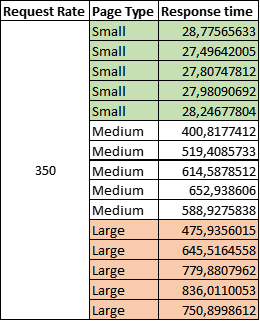
\includegraphics[width=0.4\textwidth]{img/ch3/doe350.png}
    \caption{Risultati per CTT 350}
\end{figure}

\begin{figure}[H]
    \centering
    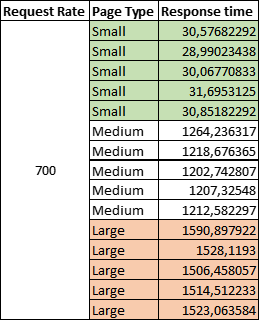
\includegraphics[width=0.4\textwidth]{img/ch3/doe700.png}
    \caption{Risultati per CTT 700}
\end{figure}

\begin{figure}[H]
    \centering
    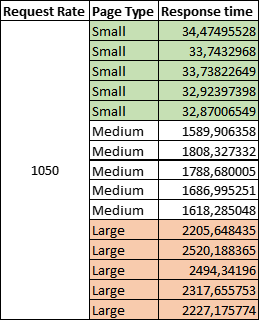
\includegraphics[width=0.4\textwidth]{img/ch3/doe1050.png}
    \caption{Risultati per CTT 1050}
\end{figure}


Successivamente, è stata effettuata una stima regressiva, il cui grafico è visibile in figura \cref{fig:modello_completo} con interazione dei fattori.

\begin{figure}[H]
    \centering
    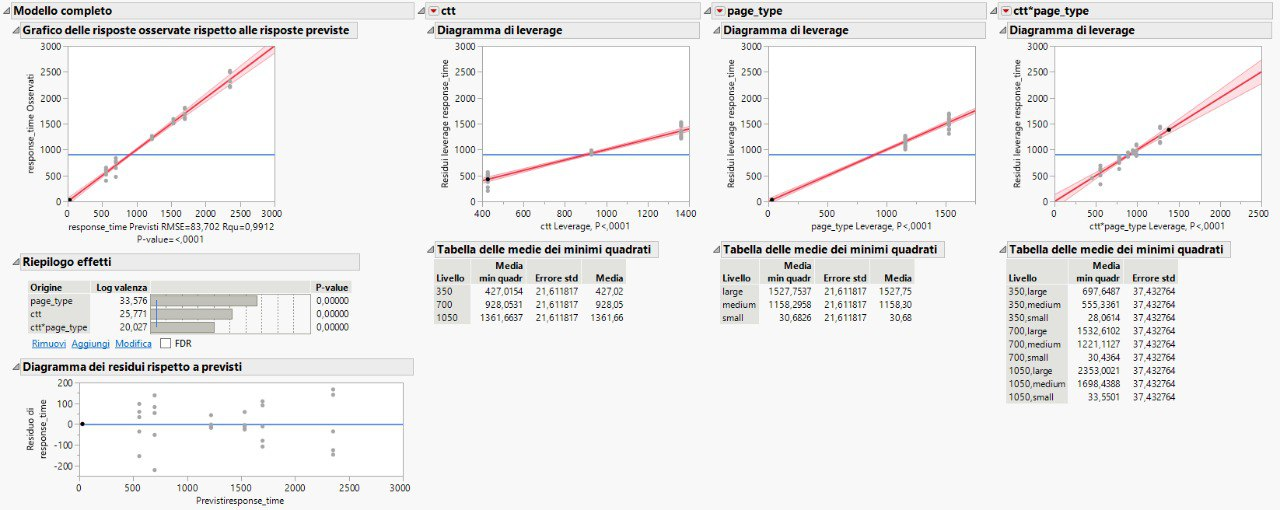
\includegraphics[width=\textwidth]{img/ch3/modello_completo.png}
    \caption{Stima del modello completo}
    \label{fig:modello_completo}
\end{figure}

In \cref{fig:analisi_varianza} e \cref{fig:test_degli_effetti}, sono riportati i dettagli del modello stimato, con la somma dei quadrati di tutti i parametri.

\begin{figure}[H]
    \centering
    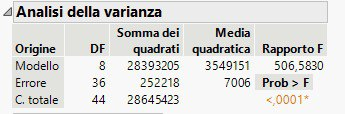
\includegraphics[width=0.6\textwidth]{img/ch3/analisi_varianza.png}
    \caption{Analisi Varianza}
    \label{fig:analisi_varianza}
\end{figure}

\begin{figure}[H]
    \centering
    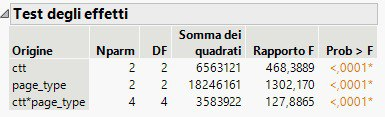
\includegraphics[width=0.6\textwidth]{img/ch3/test_degli_effetti.png}
    \caption{Test degli Effetti}
    \label{fig:test_degli_effetti}
\end{figure}

\paragraph{Importanza}
Un fattore è importante se esprime una buona
percentuale di variazione rispetto alla variazione totale del sistema.
L’importanza di un fattore si ottiene come rapporto tra
e quella del singolo fattore la somma dei quadrati totale.


Definendo come:
\begin{itemize}
    \item SSA: la devianza spiegata dal  Request Rate;
    \item SSB: la devianza spiegata dal Page Type;
    \item SSAB: la devianza spiegata dall’iterazione tra Page Size e Request Rate;
    \item SSE: la devianza spiegata dall’errore;
Si calcola la percentuale di variazione dovuta attribuita ai vari fattori, essa coincide con l'importanza del fattore stesso:
\end{itemize}

In \cref {eq:imp_ctt}, è mostrato il calcolo dell'importanza per il \textit{Request rate}:
\begin{equation}
    \frac{SSA}{SST}= \frac{6551755}{28645423} \approx 22.8\% 
    \label{eq:imp_ctt}
\end{equation}

In \cref {eq:imp_pt}, è mostrato il calcolo dell'importanza per il \textit{Page type}:
\begin{equation}
    \frac{SSB}{SST}= \frac{18246161}{28645423}  \approx 63.6\%
    \label{eq:imp_pt}
\end{equation}

In \cref {eq:imp_int}, è mostrato il calcolo dell'importanza per l'interazione tra i due fattori:
\begin{equation}
    \frac{SSAB}{SST} = \frac{3565517}{28645423}  \approx 12.4\%
    \label{eq:imp_int}
\end{equation}

In \cref {eq:imp_err}, è mostrato il calcolo dell'importanza per l'errore:
\begin{equation}
    \frac{SSE}{SST}=\frac{281990}{28645423}  \approx 1\%
    \label{eq:imp_err}
\end{equation}

Il fattore più importante risulta quindi essere il \textit{Page type}, ma anche il \textit{Request Rate} e l'inteaezione tra questi due non sono trascurabili.

\paragraph{Significatività}
Si definisce significatività di un fattore la varianza spiegata dal fattore rispetto all’errore. La significatività è un concetto statistico e quindi non è soggetta a valutazioni soggettive.

Per valutare la significatività dei fattori è possibile utilizzare diverse tipologie di test, mostrate in figura \cref{tab:anova}, a seconda della normalità dei residui e della loro omoschedasticità.

\begin{table}[H]
\centering
    \begin{tabular}{|c|c|c|}
    \hline
    \multicolumn{1}{|c|}{\textbf{Normalità}} &
    \multicolumn{1}{|c|}{\textbf{Omoschedasticità}} &
    \multicolumn{1}{|c|}{\textbf{ANOVA}}
    \tabularnewline \hline

Si & Si & F-test \tabularnewline \hline
No & Si & Kruksal-Wallis test\tabularnewline \hline
Si & No &  Welch’s test \tabularnewline \hline
No & No & Kruskal-Wallis o Friedman \tabularnewline \hline
\end{tabular}
\caption{Tabella test da applicare in base a normalità e omoschedasticità dei residui}
\label{tab:anova}
\end{table}

\paragraph{Normalità dei residui}
Come mostrato in \cref{fig:qqplot_residui}, la distribuzione dei residui, per entrambi i fattori, esce dalle bande di confidenza di una distribuzione normale.

\begin{figure}[H]
    \centering
    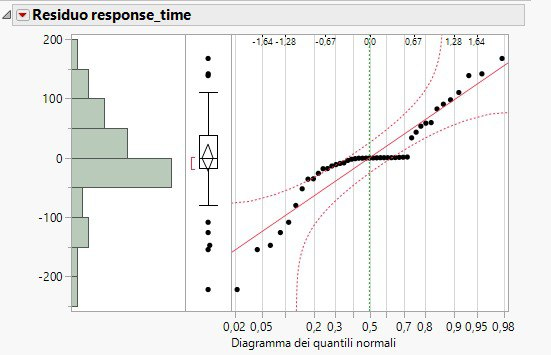
\includegraphics[width=0.8\textwidth]{img/ch3/qqplot_residui.png}
    \caption{Test di normalità dei residui}
    \label{fig:qqplot_residui}
\end{figure}


\paragraph{Omoschedasticità dei residui}
Come mostrato in \cref{fig:homo_residui}, la dispersione dei punti, per entrambi i fattori, dello \textit{scatter plot} non è costante, per cui è possibile rifiutare l’ipotesi di omoschedasticità degli errori. Oltre alla verifica visiva, è possibile affermare la non omoschedasticità dei residui attraverso il test di \textit{Levene}.

\begin{figure}[H]
    \centering
    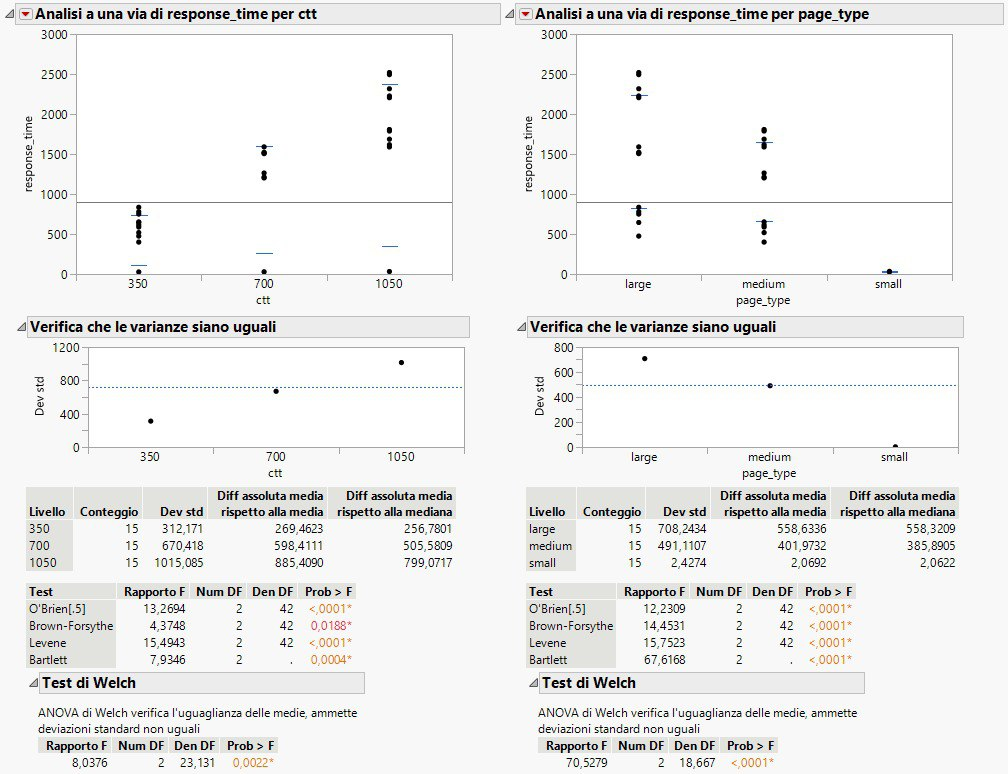
\includegraphics[width=\textwidth]{img/ch3/omoschedasticita_residui.png}
    \caption{Test di omoschedasticità dei residui}
    \label{fig:homo_residui}
\end{figure}


\paragraph{Test di significatività}

Dato che per entrambi i fattori risultano residui non normali e non omoschedastici, si è scelto di utilizzare il Test di \textit{Wilcoxon/Kruskal-Wallis}.

\begin{figure}[H]
    \centering
    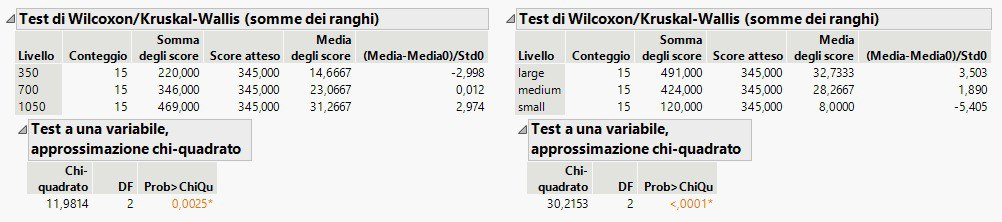
\includegraphics[width=\textwidth]{img/ch3/significativita.png}
    \caption{Test di significavità}
    \label{fig:significativita_fattori}
\end{figure}

Come mostrato in \cref{fig:significativita_fattori}, entrambi i fattori, \textit{Request Rate} e \textit{Page Size} risultano significativi a livello statistico.











